\subsection{Κατανόηση Αλγορίθμου}
Ο αλγόριθμος της διχοτόμου (με παραγώγιση) διαφοροποιείται από τον απλό μόνο στο κομμάτι 
επιλογής χωρίου αναζήτησης. Εδώ υπολογίζουμε την παράγωγο της συνάρτησης στο σημείο
διχοτόμησης και ανάλογα με το αν είναι θετική ή αρνητική επιλέγω το αριστερό ή το δεξί
διάστημα ως νέο διάστημα αναζήτησης.  
\subsection{Βήματα Αλγορίθμου}
Όμοια με τον αλγόριθμο της διχοτόμου.
\subsection{Υπολογισμοί αντικειμενικής συνάρτησης συναρτήσει του $l$}

\begin{figure}[H] % h for 'here', you can also use t (top), b (bottom), or p (page)
    \centering
    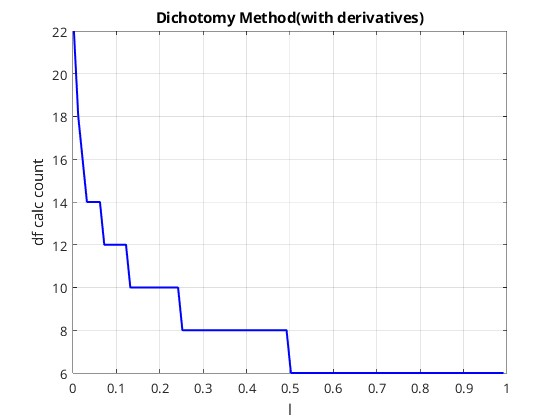
\includegraphics[width=0.5\textwidth]{media/dichotomy2f1_1} % Image file without extension
    \caption{Συνάρτηση $f_1$}
\end{figure}

\begin{figure}[H] % h for 'here', you can also use t (top), b (bottom), or p (page)
    \centering
    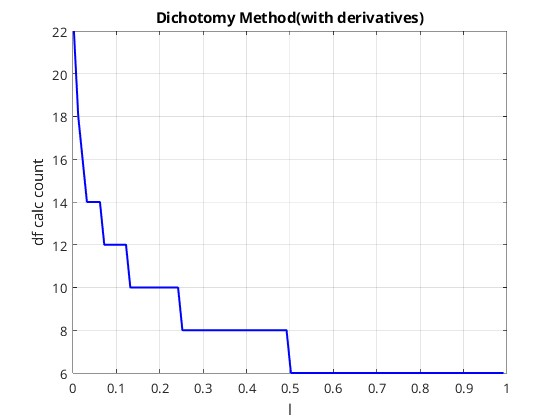
\includegraphics[width=0.5\textwidth]{media/dichotomy2f2_1} % Image file without extension
    \caption{Συνάρτηση $f_2$}
\end{figure}

\begin{figure}[H] % h for 'here', you can also use t (top), b (bottom), or p (page)
    \centering
    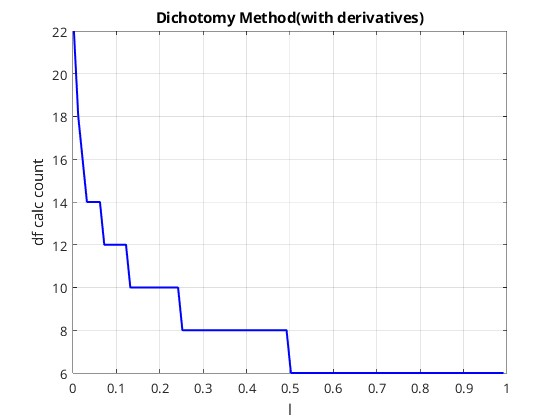
\includegraphics[width=0.5\textwidth]{media/dichotomy2f3_1} % Image file without extension
    \caption{Συνάρτηση $f_3$}
\end{figure}

\subsection{Άκρα του διαστήματος αναζήτησης συναρτήσει του δείκτη επαναλήψεων}
Συνάρτηση $f_1$:
\begin{figure}[H] % h for 'here', you can also use t (top), b (bottom), or p (page)
    \centering
    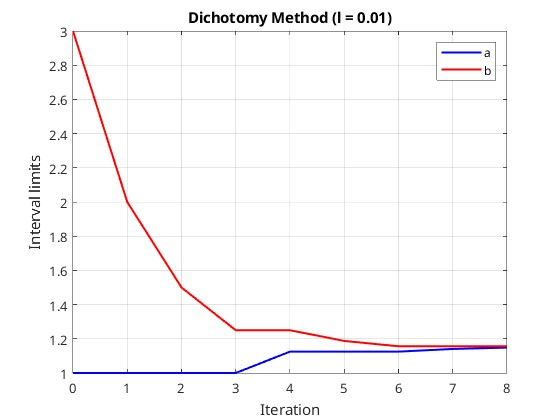
\includegraphics[width=0.5\textwidth]{media/dichotomy2f1_2001} % Image file without extension
    \caption{Συνάρτηση $f_1$}
\end{figure}
\begin{figure}[H] % h for 'here', you can also use t (top), b (bottom), or p (page)
    \centering
    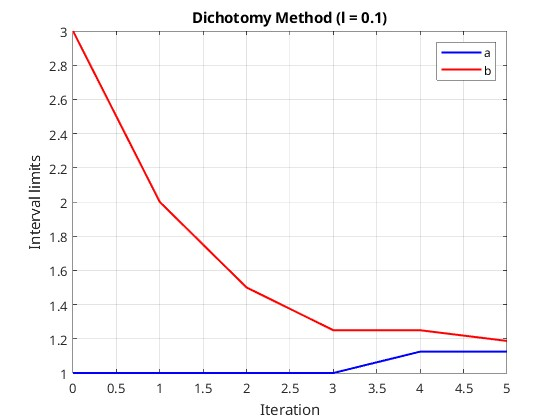
\includegraphics[width=0.5\textwidth]{media/dichotomy2f1_201} % Image file without extension
    \caption{Συνάρτηση $f_1$}
\end{figure}
\begin{figure}[H] % h for 'here', you can also use t (top), b (bottom), or p (page)
    \centering
    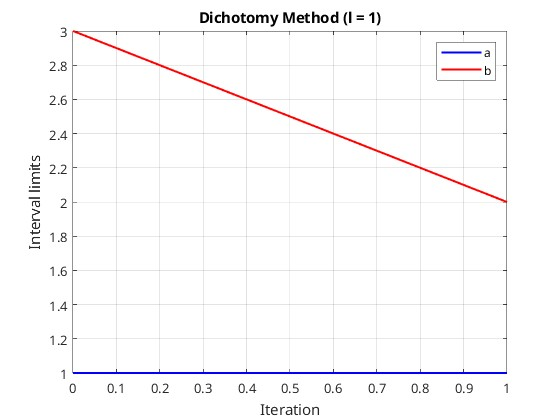
\includegraphics[width=0.5\textwidth]{media/dichotomy2f1_21} % Image file without extension
    \caption{Συνάρτηση $f_1$}
\end{figure}

Συνάρτηση $f_2$:
\begin{figure}[H] % h for 'here', you can also use t (top), b (bottom), or p (page)
    \centering
    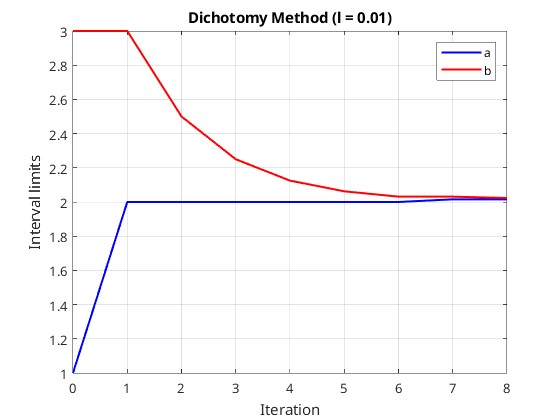
\includegraphics[width=0.5\textwidth]{media/dichotomy2f2_2001} % Image file without extension
    \caption{Συνάρτηση $f_2$}
\end{figure}
\begin{figure}[H] % h for 'here', you can also use t (top), b (bottom), or p (page)
    \centering
    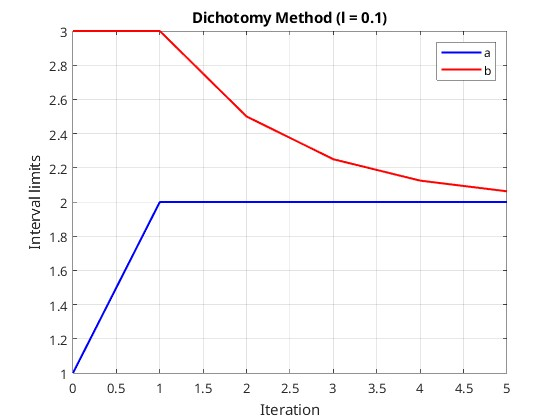
\includegraphics[width=0.5\textwidth]{media/dichotomy2f2_201} % Image file without extension
    \caption{Συνάρτηση $f_2$}
\end{figure}
\begin{figure}[H] % h for 'here', you can also use t (top), b (bottom), or p (page)
    \centering
    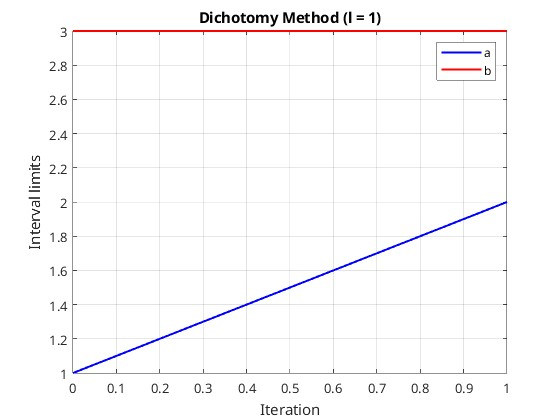
\includegraphics[width=0.5\textwidth]{media/dichotomy2f2_21} % Image file without extension
    \caption{Συνάρτηση $f_2$}
\end{figure}

Συνάρτηση $f_3$:
\begin{figure}[H] % h for 'here', you can also use t (top), b (bottom), or p (page)
    \centering
    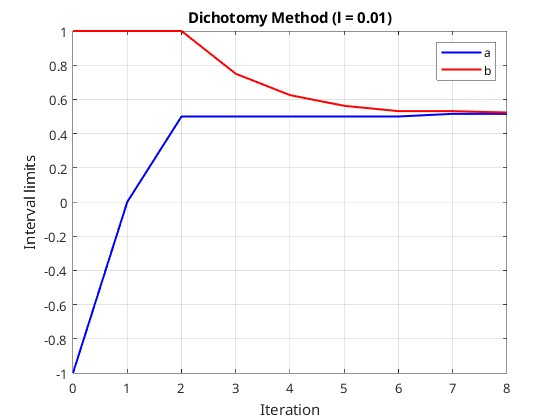
\includegraphics[width=0.5\textwidth]{media/dichotomy2f3_2001} % Image file without extension
    \caption{Συνάρτηση $f_3$}
\end{figure}
\begin{figure}[H] % h for 'here', you can also use t (top), b (bottom), or p (page)
    \centering
    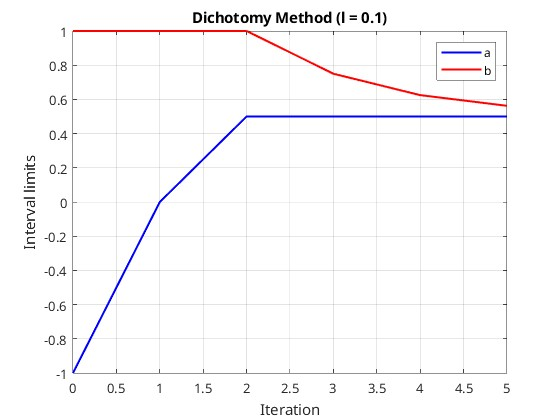
\includegraphics[width=0.5\textwidth]{media/dichotomy2f3_201} % Image file without extension
    \caption{Συνάρτηση $f_3$}
\end{figure}
\begin{figure}[H] % h for 'here', you can also use t (top), b (bottom), or p (page)
    \centering
    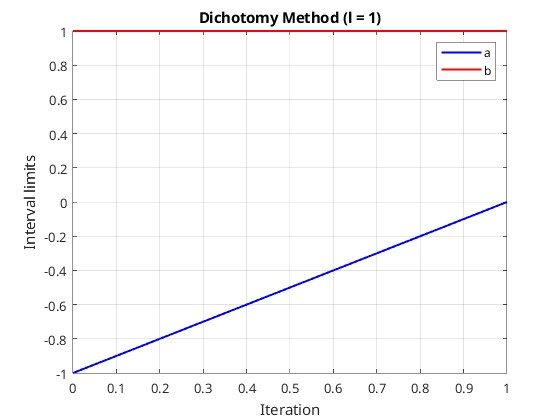
\includegraphics[width=0.5\textwidth]{media/dichotomy2f3_21} % Image file without extension
    \caption{Συνάρτηση $f_3$}
\end{figure}